\documentclass[5p,sort&compress]{elsarticle}
\usepackage{kotex}
\usepackage{pdfpages}
\usepackage{subfigure}
\usepackage{amssymb}    % Mathematical symbols
\usepackage{amsmath}    % More options for mathematics
%\usepackage{subfigure}  % More options for figures
\usepackage{epstopdf}   % Convert eps to pdf
\usepackage[separate-uncertainty=true]{siunitx}   % Proper formatting of units in math mode
\usepackage{color}      % Supports text color if needed
\usepackage{soul}       % https://ctan.org/pkg/soul
\usepackage{lmodern}    % Loading fonts
\usepackage{hyperref}   % To insert clickable references/urls
\usepackage{listings}   % To input code in the text
\usepackage{amsmath}
\usepackage{amsmath}
\usepackage{amssymb}
\usepackage{graphicx}
\usepackage{blindtext}
\usepackage{epstopdf}
\usepackage{booktabs}
\usepackage{caption}
\usepackage{subcaption}
\usepackage{cleveref}
\usepackage{mathtools}
\usepackage{pgfplots}
\usepackage{float}
\pgfplotsset{compat=newest}

\usepackage{url}
\usepackage{tikz}
\usetikzlibrary{positioning,arrows}
\usepackage{tikz}
\usetikzlibrary{positioning,arrows}
\tikzset{
block/.style={
  draw, 
  rectangle, 
  minimum height=1.2cm, 
  minimum width=1.5cm, align=center
  }, 
line/.style={->,>=latex'}
}
\usepackage{circuitikz}
\setlength{\parskip}{1em}
\newcommand{\stirlingii}{\genfrac{\{}{\}}{0pt}{}}
% Choose the style of the reference list (do not change)
\bibliographystyle{elsarticle-num}

\journal{ }
\usepackage{etoolbox}
\makeatletter
\patchcmd{\ps@pprintTitle}% <cmd>
  {Preprint submitted to}% <search>
  {Electronics and Measurement Techniques for Science and Engineering}% <replace>
  {}{}% <succes><failure>
\makeatother

% Begin the document

\usepackage{etoolbox}
\usepackage[noindentafter]{titlesec}
\titleformat{\subsection}[block]{ \itshape}{}{0em}{\filright}
\titleformat{\subsubsection}[runin]{ \itshape}{}{2em}{\filright}

\begin{document}

\begin{frontmatter}
    \title{{\LARGE Studies on Thermoelectric Properties of Thermistor and Square Platinum Plate Resistor}
    \\  {\normalsize Group 17 : Lab Module 1}
    }

    \author[1]{Junhee Myong}
    \author[2]{Jaehwan Kim}
    \author[3]{Hyemin Lee}
    \author[4]{Taehyeok Kim}
    \address[1]{College of Liberal Studies, Seoul National University, Seoul 08858 Korea}
    \address[2]{Department of Physics \& Astronomy, Seoul National University, Seoul 08858 Korea}   
    \address[3]{Department of Physics \& Astronomy, Seoul National University, Seoul 08858 Korea}    
    \address[4]{School of Earth \& Environmental Sciences, Seoul National University, Seoul 08858 Korea}    
    \date{}
    \begin{abstract}
        In this paper, we conducted several experiments, including measuring the resistance of a thermistor and platinum plate using by measuring voltage drop between both ends of a thermistor. After understanding basic properties of AD2 and methods of measuring using AD2, we could conduct 3 main experiments; measuring resistance of a thermistor considering the order of connections, measuring resistance of a square platinum plate, and observing resistance variations of a thermistor when exposed at different temperatures. After the experiment, we suggested several limitations of measuring resistance using AD2.
    \end{abstract}


\end{frontmatter}

%% How to make a heading and divide the documents into different sections

\section{Introduction} \label{introduction}
Evaluating resistance of devices is the basis of conducting experiments related to electromagnetism.
One of our goals in the experiments was measuring resistance of thermistor and platinum plate. 
A thermistor is a device that its resistance is dependent of temperature. If we assume that the thermistor’s resistance changes linearly with temperature \footnote {available when temperature change is small. That is this relation is 1st-order approximation} then,							
\begin{equation} \label{eq1}
    {\Delta}R= k(1+k{\Delta}T)
\end{equation}
where ${\Delta} R$ is change in resistance, ${\Delta} T$ in change in temperature and $k$ is the first-order temperature coefficient of resistance. Thanks to the thermoelectric property of it we can briefly observe this in our third experiment.  
\newline
Resistance can be obtained by Ohm’s law, $R = V/I$. However, Ohm’s law is available when the settings and devises fulfill an Ohmic regime. So firstly, we should check whether our designs follow Ohmic regime. and we could calibrate the offsets of data. When we measure resistance with high precision, we avoid using a multimeter which is based on 2-terminal method because of the obvious flaws of it. For example, it might have relatively high contact resistance to gain the precise quantity with low errors. Therefore, we should experiment with other methods like 4-terminal method and van der Pauw method.  
\newline
\begin{figure}[h]
\centering
    \subfigure{
        \begin{circuitikz}[scale=0.5,transform shape] 
        \draw (0,0) to[R, l=$R_0  (DUT)$] (0,6)  to[R, l=$r_1$] (3,6) to[voltmeter] (3,0) to[R, l=$r_2$] (0,0);
        \draw (3, 6) -- (5, 6) to[american voltage source] (5, 0) -- (3, 0);
        \end{circuitikz}
    }
    
    \subfigure{
        \begin{circuitikz}[scale=0.5,transform shape] 
        \draw (0, 0)  to[R, l_=$R_0 (DUT)$] (0, 6) to[R, l_=$r_1$] (3, 6) to[voltmeter] (3, 0) to [R, l=$r_2$] (0,0);
        \draw (0,6) -- (0, 7) to[R, l_=$r_3$] (3, 7) -- (5,7) to[american voltage source]  (5,-1) -- (3,-1) to[R, l=$r4$] (0,-1) --(0,0);
        \end{circuitikz}
        %이 부분에 문제가 있었습니다
        %\caption{2-terminal method} 
        %\label{fig:expcircuit2}  
    }
    \caption{4 -terminal method}
    \label{fig:exp1circuit}
\end{figure}

Because we used the device, Analog Discover2(AD2) which has only voltage source, we should devise a method that can measure resistance without current source with reliability. AD2 is a powerful devise that contains DC voltage source, digital oscilloscope and voltmeter. But to fully use these functions, we should devise a programmable system so that the outcome values or inputs of the device under test (DUT) are reliable. After some efforts to design the program and fix it, we are finally ready to conduct experiments.

In this paper we present analysis results from three experiments. As mentioned earlier, through those we can consider critically how to measure more accurately in electromagnetic experiments. As a part of our experiments we also examine thermoelectric property of thermistor by cooling water with ice.


\section{Methods}
\subsubsection{Pre-experiment : Studies on AD2}

\begin{figure}[h]
\centering
    \subfigure[Thermistor connected far from ground]{
        \centering
        \begin{circuitikz}[scale=0.6,transform shape] 
        \draw (0,0) to[american voltage source] (0,6)--(3,6) to[R, l_=Known resistor] (3,3) to[R, l_=DUT] (3,0) -- (0,0);
        \draw (3,2.5) -- (4,2.5) to[voltmeter] (4,0.5) -- (3,0.5);
        \draw (3, 6) -- (5, 6) to[voltmeter] (5, 0) -- (3, 0);
        \end{circuitikz}
        \label{fig:exp1circuit}
        }
    \subfigure[Thermistor connected close to ground]{
        \begin{circuitikz}[scale=0.6,transform shape] 
        \draw (0, 0) -- (3, 0) to[R, l_=DUT] (3, 3) to[R, l_=Known resistor] (3, 6) -- (0, 6) to[american voltage source] (0, 0);
        \draw (3,2.5) -- (4,2.5) to[voltmeter] (4,0.5) -- (3,0.5);
        \draw (3, 6) -- (5, 6) to[voltmeter] (5, 0) -- (3, 0);
        \end{circuitikz}
        \label{fig:expcircuit2}
    }
    \caption{Circuit diagrams used in experiment}
\end{figure}
.
\newline
After conducting experiment 1 which was about measuring resistance of a thermistor, we found out that one of two channels of oscilloscope has a wrong zero-point. We could test out the error by measuring voltages between two points with no external voltages with the oscilloscope channel. So we had to calibrate the zero-point using the WaveForms software. After the calibration, we conducted the experiment again.
 
\subsubsection{Experiment 1 : Thermistor resistance measurement}
.\newline
After setting up AD2, we built up the circuit as Fig.2, to measure the resistance of a thermistor. The input voltage was given by WaveForms software, and the measurement through oscilloscope was also executed by the WaveForms software. We gave the input voltage as a form of triangle wave which amplitude was 1(V), which is small enough to fit inside the measuring range of the oscilloscope, and period of 5 seconds. The period is long enough to consider the entire circuit current as DC. The form of wave is necessary because we used two voltage measurements; between both sides of the thermistor and the entire circuit, to calculate the resistance of the thermistor. When the wave is triangular, the ratio between two voltages($V_{DUT}$-$V_{tot}$ graph slope) is constant, which makes it easier to calculate the resistance of the thermistor. We chose the load resistor  with a sufficiently large resistance to satisfy the approximate condition, but not too large, because it induces low precision in measuring $V_{DUT}$.
equation to obtain the resistance value of the thermistor($R_{t}$) is given below, where $R_{L}$ is the resistance of the load resistor, and r is the equivalent resistance of the wire. Also, $V$ is the voltage given at both sides of the entire circuit, and $V_{DUT}$ is the voltage measured at both sides of the thermistor(DUT).

\begin{equation}\label{eqfitting}
    I = \frac{V_{tot}-V_{DUT}}{R_{L}}
\end{equation}
\begin{equation}\label{eqfitting}
    R_{t} = \frac{V_{DUT}}{I}=\frac{R_{L}}{\frac{V_{tot}}{V_{DUT}}-1}
\end{equation}

The 2 channels of oscilloscope each measured $V_{DUT}$ and $V_{tot}$. So we could derive the I-V graph, and the slope of the linear approximation of the graph would be resistance of the thermistor.

However, there is a serious problem. When the load resistor has enough resistance to be comparable with the impedance of AD2, the connection order becomes important. This is because the ideal voltmeter must have infinite resistance to measure the voltage correctly. However, because  For this reason, we chose [1$M\Omega$] resistor as the load resistor and designed the circuit in 2 ways; connecting thermistor near the ground of the circuit as Fig. 2a, and connecting thermistor far from the ground of the circuit as Fig. 2b. 
Also, to find out the impedance of the AD2 voltmeter, we connected 10(k$\Omega$) resistor instead of thermistor near the ground of the circuit and near the cathode of the circuit. Related equations are given below. $R_{1}$ and $R_{2}$ are the internal resistance of the oscilloscope. Through some calculation, $R_{tot}$ can be expressed in terms of ${R'}_{L} = \frac{R_{osc}R_{L}}{R_{osc}+R_L}$ with $R_{osc} = R_1 + R_2$
%멀때
\begin{equation}\label{eq:Impedance}
    V_{measure} = V_{tot}\frac{R_{DUT}}{R_{DUT}+R'_L}
\end{equation}

In the same way, $V_{measure}$ can be obtained in the circuit of Figure.\ref{fig:exp1circuit} as follows where $R'_{DUT}$ = $R_{DUT}R_{osc}/(R_{DUT}+R_{osc})$
%가까울때
\begin{equation}\label{eq:Impedance_R_DUT}
    V_{measure} = V_{tot}\frac{R'_{DUT}}{R'_{DUT}+R_L}
\end{equation}

These two calculations match with the circuit of Figure 3 mentioned below.

\begin{figure}[h]
    \centering
    \subfigure[This time, thermistor(DUT) is connected close to the ground. It is evident from the equations that this makes less voltage measurement error.]{
    \begin{circuitikz}[scale=0.6,transform shape]
	    \draw (0,0) -- (1.5, 0) to[R = load] (3,0)	to[R = DUT] (5,0) -- (8,0) node[ground] {};
	    \draw (3,0) -- (3,2) -- (5, 2) to[R=$R_{1}$] (6.5, 2) to[R=$R_{2}$] (8,2) -- (8, 0);
	    \draw (5, 0) -- (5, 1) to[R=$R_{1}$] (6.5, 1) to[R=$R_{2}$] (8, 1);
	    \draw (6.5, 2) to[voltmeter] (6.5, 1);
	    \filldraw (6.5, 1) circle [radius = 0.05] node [below]{$b$};
	    \filldraw (6.5, 2) circle [radius = 0.05] node [above]{$a$};
    \end{circuitikz}
    }
    \subfigure[This time, thermistor(DUT) is connected far from the ground. It is evident from the equations that this makes more voltage measurement error.]{
    \begin{circuitikz}[scale=0.6,transform shape]]
    	\draw (0,0) -- (3, 0) to[R = DUT] (5,0)	to[R = load] (6.5,0) -- (8,0) node[ground] {};
    	\draw (3,0) -- (3,2) -- (5, 2) to[R=$R_{1}$] (6.5, 2) to[R=$R_{2}$] (8,2) -- (8, 0);
    	\draw (5, 0) -- (5, 1) to[R=$R_{1}$] (6.5, 1) to[R=$R_{2}$] (8, 1);
    	\draw (6.5, 2) to[voltmeter] (6.5, 1);
	    \filldraw (6.5, 1) circle [radius = 0.05] node [below]{$b$};
	    \filldraw (6.5, 2) circle [radius = 0.05] node [above]{$a$};
    \end{circuitikz}
    }
    \caption{Two methods of connecting thermistor(DUT). We chose to connect DUT close to the ground because it makes less voltage measurement error due to the impedance of AD2.}
    \label{fig:whatever}
\end{figure}

\subsubsection{Experiment 2 : Platinum plate resistance measurement}
.\newline
The next experiment uses same circuit, but with a platinum plate resistor instead of thermistor. The structure and shape of the platinum plate resistor are shown below(Figure 4).

\begin{figure}[h]
\centering
\subfigure[Shape of the plate resistance]{
\includegraphics[width=.225\textwidth]{Plate.jpg}
}
\subfigure[Simplified structure of the plate resistance measure device]{
\includegraphics[width=.225\textwidth]{Plate_structure.jpg}
}
\caption{This figure shows the shape and overall structure of the plate resistance used in experiment 2.}
\label{fig:DUT_curve}
\end{figure}

In this experiment, the input voltage is given between the top two vertexes and we measure the voltage between the lower two vertexes. Just like experiment 1, we measured the resistance using the slope of V-V graph. After the measurement, we compared the result with our theoretical predictions.

\subsubsection{Experiment 3 : Observing thermoelectric property of a thermistor}
.\newline
In this session we repeated experiment 1, but with thermistor exposed in different temperature environments. Due to the absence of thermometer and heating devices, we used cold water with ice to lower the temperature, and observed how resistance of the thermistor changes. Other conditions were exact same with experiment 1. Because the thermistor is a semiconductor, it would likely have negative temperature coefficient, meaning that the resistance would decrease in higher temperature. After exposing the thermistor at room temperature long enough, we put the thermistor end at warm water to heat the thermistor, and added ice to cool.


\section{Results} 


\subsubsection{Experiment 1}.
\newline{}
Figure.\ref{fig:averagedVIdata1} shows the measured data of $V_{DUT}$ according to $V_{tot}$ in the circuit in which the DUT is set as the thermistor in Figure \ref{fig:expcircuit2}. When $V_{input}$ increases and decreases, the relative error of the slopes and the absolute error of the y-intercepts are less than $10^{-4}$, 0.1[mV] respectively. Linear regression line between $V_{DUT}$ and $I_{DUT}$ is shown in Figure.\ref{fig:regressedVIdata}.

\begin{figure}[h]
\centering
\subfigure[correlation between $V_{DUT}$ and $V_{tot}$]{
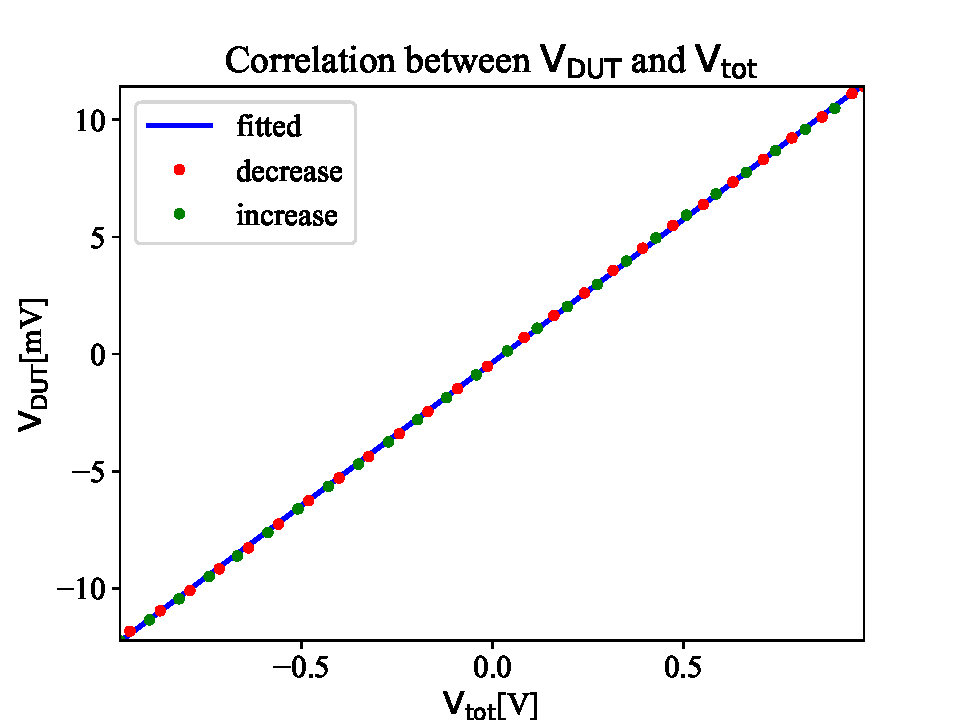
\includegraphics[width=.4\textwidth]{0_VV_curve_with_calibration.pdf}
\label{fig:averagedVIdata1}
}
\subfigure[correlation between $V_{DUT}$ and $I_{DUT}$]{
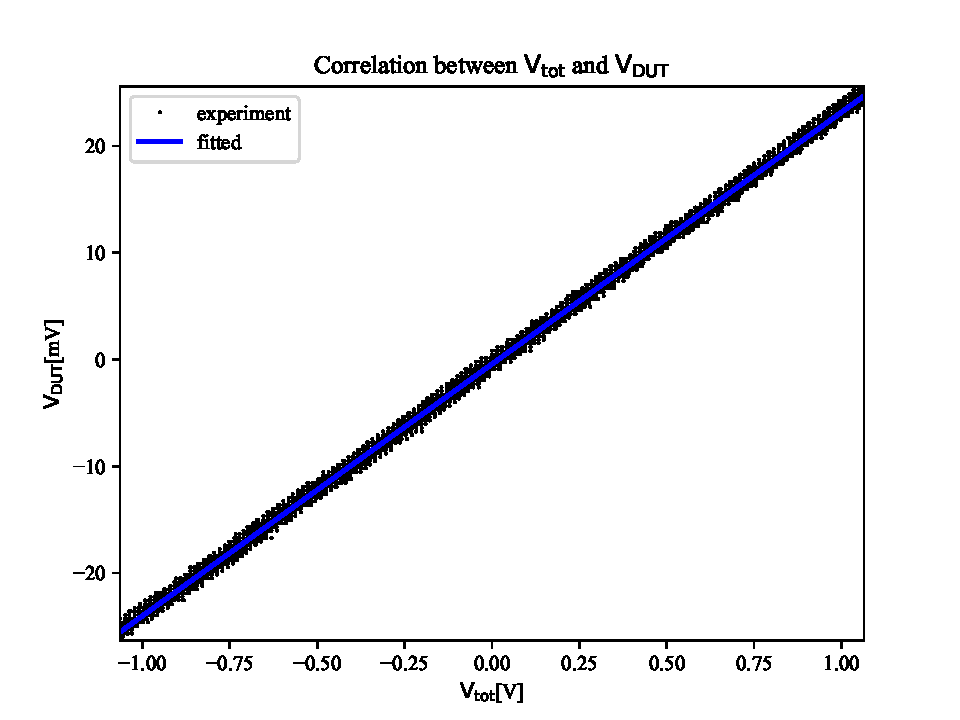
\includegraphics[width=.4\textwidth]{0_IV_curve_with_calibration.pdf}
\label{fig:regressedVIdata}
}
\caption{
For the legibility of the graph, we replaced 100 consecutive data points in time with the mean value for a one period of a triangular wave when plotting. The equation of linearly fitted line in (b) is $y = 12.32[k\omega]x - 0.4[mV]$ with $r^2 = 0.995$} 

\label{fig:VVcurve}
\end{figure}

Note that in the figures including linear regression below, all data points are preprocessed with 100-average as above Figure.\ref{fig:VVcurve}.
%y = (-0.000427) + (24141.537045)
%r^2 = 0.998701

For the linear regression, the error of the y-intercept is about 1[mV], which is comparable to y-intercept. So the y-intercept can be ignored.
$R_{th}$ can be obtained as 12.32[k$\Omega$] directly through the slope in Figure\ref{fig:regressedVIdata}.
\newline{}
When the thermistor is connected far from the ground, the resistance is calculated as 24[k$\Omega$] in the same way as above. This result deviates by almost twice the true value due to the oscilloscope's impedance as seen in \ref{} eq적어주세요 여러분...

Now consider the oscilloscope's impedance $R_{osc}$. In the circuit in which the DUT of Figure.\ref{fig:exp1circuit} is set to 10k Ohm, the measurement results of $V_{measure}$ according to $V_{tot}$ and linear regression of them are shown in Figure.\ref{fig:Impedance_VV}.

\begin{figure}[h]
\centering
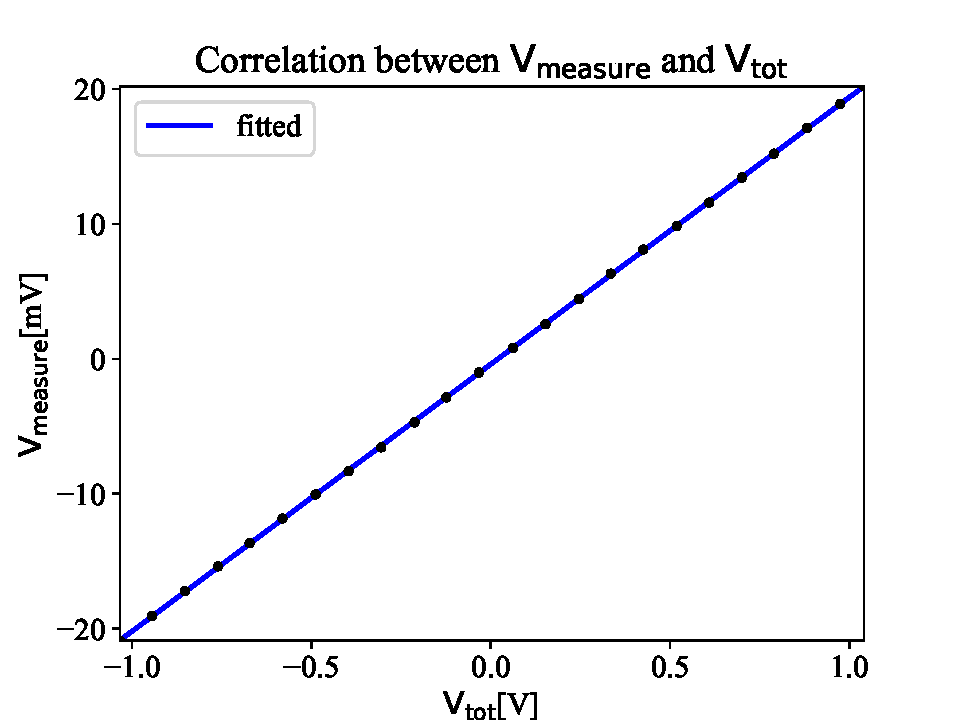
\includegraphics[width=.5\textwidth]{Impedance_VV.pdf}
\caption{The equation of linearly fitted line is $y = 0.019[-]x - 0.4[mV]$ with $r^2 = 0.9993$}
\label{fig:Impedance_VV}
\end{figure}

From Equation.\ref{eq:Impedance}, $R'_L = R_{DUT}(1-B)/B = 495[k\Omega]$ can be obtained by using the slope B in Figure.\ref{fig:VVcurve}. Resistance of $R_{osc} = 981[k\Omega]$ was obtained directly from the definition of $R'_L$. The relative error is $6[\%]$ which is obtained by comparison with $R_{{osc}_{theory}}$.
%이거 레퍼런스에 달아주세요. AD2 8페이지의 세 저항의 값을 더하면 됩니다. 이 내용을 introduction에 적어주세요. $R_{osc}_{theory}$ = 1.04[MOhm]
Let's correct the Resistance $R_{th}$ obtained above by considering $R_{osc}$. Equation.\ref{eq:Impedance_R_DUT} gives a exact form of $V_{measure}$. And the current $I = (V_{tot}-V_{measure})/R_{L}$ used in the linear regression above is as follows.
\begin{equation}
    I = \frac{V_{tot}}{R_L + R'_{DUT}}
\end{equation}
Therefore, the slope of the above linear regression line is exactly $R'_{DUT}$. From the definition of $R'_{DUT}$,
\begin{equation}
    R_{{th}_{correction}} = \frac{R'_{DUT}R_{L}}{R_L - R'_{DUT}} = 12.47[k\Omega]
\end{equation}


\subsubsection{Experiment 2}.
\newline{}
The data obtained by measuring $V_{DUT}$ for the current $I_{input}$ flowing through AB is shown in Figure.\ref{fig:ABDC}. $R_{AB, DC} = 2.325[Omega]$ is the slope of the line in the Figure.

\begin{figure}[h]
\centering
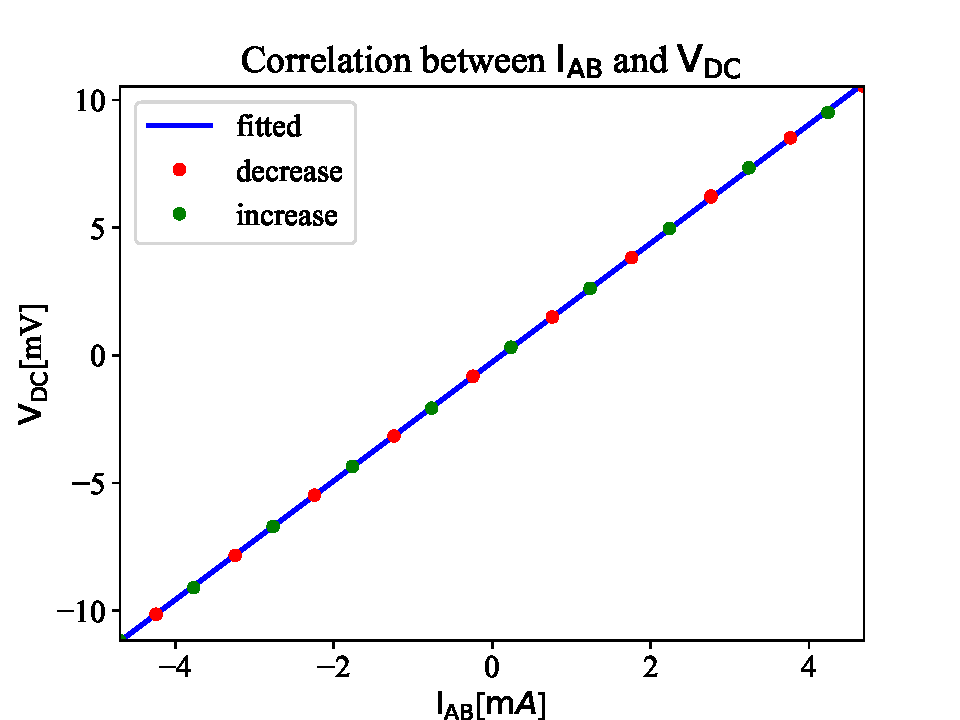
\includegraphics[width=.5\textwidth]{platinum_ABDC_VI.pdf}
\caption{The equation of linearly fitted line is $y = 2.325[\Omega]x - 0[mV]$ with $r^2 = 0.9997$}
\label{fig:ABDC}
\end{figure}
%return{
%y = (-0.000267) + (2.325276) * x\newline{}
%$r^2$ = 0.999685  
%$R_{DUT}$ = 2.3252758847205217  
%}
In the Figure, there is no difference between when current flows in the forward direction and when it flows in the reverse direction. Therefore we did not regress separately when the direction of the current is changed, but further regressed the following three cases and obtained resistances from the slopes as below.
\begin{align*}
    &R_{DC, AB} = 2.39[\Omega]\\
    &R_{BC, AD} = 4.49[\Omega]\\
    &R_{AD, BC} = 4.56[\Omega]
\end{align*}
Therefore, $R_{horizontal}$ and $R_{vertical}$ are given as follows.
\begin{align*}
&R_{horizontal} = 2.36[\Omega]\\
&R_{vertical} = 4.53[\Omega]
\end{align*}
By the Equation.\ref{vanderpauw_rho}, $R_{S}$ = 15.06[$\Omega$]. As a consequence, $\rho$ are given as follows.
\begin{equation}
    \rho = R_{S} * t = 3.01*10^{-7}[\Omega m]
\end{equation}

The theoretical value could be calculated from Equation.\ref{eq:} 
\begin{equation}
    {\rho}_{theory} = asdfasdfasdfasdfasdf
\end{equation}
%introduction에 추가해주세요
So we have a Relative error of $\rho$ = ()$\%$

\subsubsection{Experiment 3}.
\newline{}
We setted $R_L$=1$[M\Omega]$ and DUT to thermistor in the circuit in Figure.\ref{fig:expcircuit2}. Instead of using a triangular wave to more effectively see the voltage that changes from time to time, the DC voltage of 1V was applied and $V_{DUT}$ was measured. $V_{DUT}$ $-$ $I_{AB}$ curve is shown in Figure.\ref{fig:cooling_VT}
\begin{figure}[h]
\centering
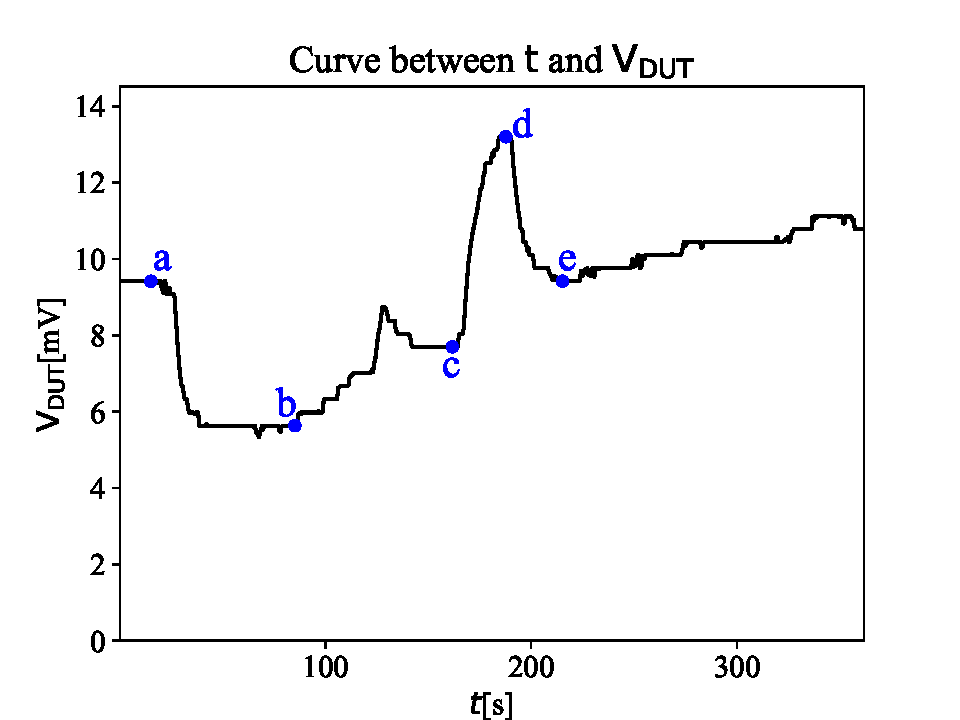
\includegraphics[width=.5\textwidth]{ICE_coolign_Vt.pdf}
\caption{ 
$V_{DUT}$ curve over time $t$. From a to e, the following actions were taken.
a : put the thermistor in the water in the bottle\\
b : put the ice in the water\\
c : move the thermistor near the ice\\
d : move thermistor away from the ice\\
e : thermistor comes out of the water
}
\label{fig:cooling_VT}
\end{figure}
When the temperature of the thermistor increased at a and d, the voltage increased, and when it decreased at b, c and e, the low voltage decreased. Therefore we can verify that the thermistor's resistance decreases as the temperature increases. 
%이거는 혜민이가 더 쓸거면 써주세요
The exponential trend of voltage from c to d and d to e will be discussed in discussion.



\section{Discussions}
\subsection{Instrument Errors}
The most important point of this experiment was the impedance of AD2 scope which approximates the load resistor's. Since the scope is grounded at the end\footnote{See AD2 reference manual, p.8}, it is not a mere resistor between two point. Rather, it consists a parallel connection which makes the effective resistance of the circuit decrease. So it is not able to measure the voltage across the load resistance without a fundamental error when we do not know the internal circuit of AD2 scope. Consider two quite similar circuits shown in Fig. ???. For the circuit (a) there are 5 different path between DUT and the ground-including the path via voltmeter-, two of them does not lies on the load. It clearly reduces the effective load resistance, making the current increase from what was calculated from the ideal oscilloscope, which causes the positive error of the DUT resistance. For the circuit (b), on the other hand, there is only one more path to affect the current of load and DUT, with rather bigger resistance, leaving relatively small(about 70\% of (a)\footnote{For (a), the current is about 2.5times of the ideal one, where the current is about 1.7times for (b)}), yet not negligible error of current. This means the resistor with smaller resistance-for now, DUT,- should be placed closer to the ground to make the error decrease when we do not know the impedane of AD2.
\newline
\begin{figure}[h]
    \centering
    \subfigure[]{
    \begin{circuitikz}[scale=1,transform shape]
	    \draw (0,0) -- (1.5, 0) to[R = DUT] (3,0)	to[R = load] (5,0) -- (8,0) node[ground] {};
	    \draw (3,0) -- (3,2) -- (5, 2) to[R] (6.5, 2) to[R] (8,2) -- (8, 0);
	    \draw (5, 0) -- (5, 1) to[R] (6.5, 1) to[R] (8, 1);
	    \draw (6.5, 2) to[voltmeter] (6.5, 1);
	    \filldraw (0, 0) circle [radius = 0.05] node [below]{$V_{in}$};
	    \filldraw (3, 0) circle [radius = 0.05] node [below]{$V_{1}$};
	    \filldraw (6.5, 1) circle [radius = 0.05] node [below]{$V_{2}$};
	    \filldraw (6.5, 2) circle [radius = 0.05] node [above]{$V_{3}$};
    \end{circuitikz}
    }
    \subfigure[]{
    \begin{circuitikz}[scale=1,transform shape]
    	\draw (0,0) -- (3, 0) to[R = load] (5,0) to[R = DUT] (6.5,0) -- (8,0) node[ground] {};
    	\draw (3,0) -- (3,2) -- (5, 2) to[R] (6.5, 2) to[R] (8,2) -- (8, 0);
    	\draw (5, 0) -- (5, 1) to[R] (6.5, 1) to[R] (8, 1);
    	\draw (6.5, 2) to[voltmeter] (6.5, 1);
    	\filldraw (0, 0) circle [radius = 0.05] node [below]{$V_{in}$};
	    \filldraw (5, 0) circle [radius = 0.05] node [below]{$V_{1}$};
	    \filldraw (6.5, 1) circle [radius = 0.05] node [below]{$V_{2}$};
	    \filldraw (6.5, 2) circle [radius = 0.05] node [above]{$V_{3}$};
    \end{circuitikz}
    }
    \caption{For (a), the load is put close to the ground and DUT is put far from the $V_{in}$, where (b) is in inverse-sequence.}
    \label{fig:whatever}
\end{figure}
\newline
For similar reason, DUT should be placed close the ground when measuring the voltage across DUT. See Fig. ???. Note that this kind of error does not stems from the resolution AD2. Since it entirely comes from the parallel connection of AD2 scope, the effect can be calculated in terms of the impedance of AD2 scope, which was measured from pre-experiment . This fact provides the basic tools for correcting the instrument bias.
\newline
\begin{figure}[h]
    \centering
    \subfigure[]{
    \begin{circuitikz}[scale=1,transform shape]
	    \draw (0,0) -- (1.5, 0) to[R = load] (3,0)	to[R = DUT] (5,0) -- (8,0) node[ground] {};
	    \draw (3,0) -- (3,2) -- (5, 2) to[R] (6.5, 2) to[R] (8,2) -- (8, 0);
	    \draw (5, 0) -- (5, 1) to[R] (6.5, 1) to[R] (8, 1);
	    \draw (6.5, 2) to[voltmeter] (6.5, 1);
	    \filldraw (0, 0) circle [radius = 0.05] node [below]{$V_{in}$};
	    \filldraw (3, 0) circle [radius = 0.05] node [below]{$V_{1}$};
	    \filldraw (6.5, 1) circle [radius = 0.05] node [below]{$V_{2}$};
	    \filldraw (6.5, 2) circle [radius = 0.05] node [above]{$V_{3}$};
    \end{circuitikz}
    }
    \subfigure[]{
    \begin{circuitikz}[scale=1,transform shape]]
    	\draw (0,0) -- (3, 0) to[R = DUT] (5,0)	to[R = load] (6.5,0) -- (8,0) node[ground] {};
    	\draw (3,0) -- (3,2) -- (5, 2) to[R] (6.5, 2) to[R] (8,2) -- (8, 0);
    	\draw (5, 0) -- (5, 1) to[R] (6.5, 1) to[R] (8, 1);
    	\draw (6.5, 2) to[voltmeter] (6.5, 1);
    	\filldraw (0, 0) circle [radius = 0.05] node [below]{$V_{in}$};
	    \filldraw (5, 0) circle [radius = 0.05] node [below]{$V_{1}$};
	    \filldraw (6.5, 1) circle [radius = 0.05] node [below]{$V_{2}$};
	    \filldraw (6.5, 2) circle [radius = 0.05] node [above]{$V_{3}$};
    \end{circuitikz}
    }
    \caption{For (a), the DUT is put close to the ground and load is put far from the $V_{in}$, where (b) is inverse-sequence.}
    \label{fig:whatever}
\end{figure}
\subsection{About Experiment 3}
In the result of experiment 3, there are three steep, exponential-like peaks; One is decreasing, when the thermistor was dipped into the warm water, and the others are increasing, when it contacted with the ice. Each one is the result of rapid change of temperature, which can be well-described by exponential function. So, even though this experiment was executed without thermometer, this peaks tells that this experiment reveals the strong relation between the temperature and the resistance of the themistor qualitatively.
\subsection{Resistivity of Thin Sample}
In experiment 2, the resistivity of Pt film was measured about thrice the bulk resistivity of Pt. Such disagreement can be explained by some models. For example, the Fuchs model based on Boltzmann model of free electrons, grain boundary scattering model suggested by Mayadas, \textbf{\textit{etc.}}. 
\newline
For 4-probe Van Der Pauw method, the contact should be on the corner of the sample. If the contact is formed inside the sample, the effective length of the sample decreases, which provokes the error in order of exponential. In this experiment, the distance between the contact and the corner of the sample was comparable to 1/10 of sample's side length, which might causes a complicated errors that involves the real resistance of the sample. Note that, however, the contact points composes a square. So the obtained sheet resistance and the resistivity still has less errors.

\subsection{Further study}
In Experiment 3, negative characteristic of thermistor was verified. Because of absence of thermometer, however, the coefficient could not be determined, leaving the characteristics of the thermistor not be constructed. So it would be recommendable to examine the thermistor quantitatively. Does the resistance of thermistor have a linear relation with the temperature for wide range? If then, what is the coefficient? If not, what kind of relation the resistance have with the temperature?
\newline
In Experiment 2, we obtained the resistivity of 20nm-Pt film, which was about thrice of the bulk resistivity of Pt. But this simple experiment is not enough to probe the models that explain the larger resistivity of thin metal film. To verify this models, we suggest a experiment that measures the rsistivity of growing-Pt film in real time. Some might have done it, but there is no sufficient data that containing the geometric configuration of the sample. It would reveal the relation between the thickness of film and the resistivity.

\section{Conclusions}
Firstly, the impedance of the AD2 scope was measured successfully; $Z_{sc} \approx 1M \Omega$. With this, we obtained some corrected data set about the resistance of the thermistor (thermistor code) and the Pt nano film, which allowed us to calculate the resistance precisely; $R_{thermistor} = ???$, $R_{s} = ???$, $\rho_{Pt film} = ???$. Especially for resistivity of the Pt nano film, we showed that the thin film has larger resistivity than the bulk. This experiment, measuring resistance in various condition, built the founding stone of electronics.

\bibliography{references}

\begin{thebibliography}{9}

\bibitem{} 
Analog Discovery $2^{TM}$ Reference Manual. Digilent, 2015
\bibitem{} 
J.R. Sambles. \textbf{\textit{The Resistivity of Thin Metal Films-Some Critical Remarks}}. Thin Solid Films, 106(1983), 321-331.
\bibitem{} 
Gert Rietveld, \textbf{\textit{et al.}}, \textbf{\textit{DC Conductivity Measurements in the Van Der Pauw Geometry}}. IEEE Transactions on Instrumentation and Measurement, Vol.52, No.2(2003), 449-453.
\bibitem{} 
Maria P. Gutierrez, Haiyong Li, Jeffrey Patton, \textbf{\textit{et al.}}, \textbf{\textit{Thin Film Surface Resitivity}}.(2002).


\end{thebibliography}


\end{document}